% !TeX encoding = UTF-8
% !TeX program = pdflatex
% !TeX spellcheck = it\_IT
\documentclass[binding=0.6cm, oneside, noexaminfo, italian]{sapthesis}
\usepackage[italian]{babel}
\usepackage[utf8]{inputenc}
\usepackage{hyperref}
\usepackage{graphicx}
\usepackage{afterpage}
\usepackage{makeidx}
\usepackage{chngcntr}
\counterwithin{figure}{section}

\renewcommand{\thesection}{\arabic{section}}
\makeindex
\newcommand\blankpage{%
    \null
    \thispagestyle{empty}%
    \addtocounter{page}{-1}%
    \newpage}


\title{4Money}

\subtitle{Gestisci il tuo portafogli in maniera smart}

\author{Cristian Andrei Mai Mihai}

\IDnumber{1942925}

\course{Corso di Laurea in Ingegneria Informatica e Automatica}

\courseorganizer{Facoltà di Ingegneria dell'informazione, informatica e statistica}

\AcademicYear{2022/2023}

\advisor{Prof. Riccardo Rosati}

\customadvisorlabel{Relatore}

\copyyear{2023}

\authoremail{cristianmm1240@gmail.com}

\begin{document}

\frontmatter
\maketitle

\afterpage{\blankpage}

\newpage

\tableofcontents

\mainmatter
\newpage

\section{Introduzione}
\subsection{Presentazione}
Questa tesi ha lo scopo di presentare 4Money, un’applicazione web nata come progetto del corso di Linguaggi e Tecnologie per il Web, descrivendo le funzionalità di tale sito sia lato client che lato server, oltre alle motivazioni che hanno portato alla scelta di certe implementazioni. \\ \\
4Money è un’applicazione web che si pone l’obiettivo di aiutare i propri utenti a gestire al meglio le proprie finanze e per raggiungerlo offre un’interfaccia interattiva e funzionale la quale consente all’utente una vasta varietà di azioni disponibili e funzioni:
\begin{itemize}
    \item Conserva informazioni riguardanti le spese o gli introiti salvati dall’utente in base a specifiche categorie, sia che questi siano passati o futuri;
    \item Permette di gestire un fondo di risparmio, detraendo o assegnando a esso risorse in base alle necessità dell’utente;
    \item Presenta diversi grafici per aiutare a visualizzare in modo rapido e intuitivo le proprie abitudini finanziarie, dalla quantità di soldi che vengono spesi durante i vari mesi dell’anno, alla percentuale per categoria delle spese del mese corrente;
    \item Completa libertà nella gestione del proprio profilo;
    \item Possibilità di esportare i dati dei propri movimenti in vari formati;
\end{itemize}
Sono presenti, inoltre, tre profili di tipo amministratore, uno per ognuno dei creatori di 4Money, per una gestione di dinamica degli utenti e delle categorie delle transazioni. In particolare, gli amministratori possono bloccare o, se ritenuto necessario, eliminare gli account degli utenti comuni; vi sono dei grafici a loro dedicati per osservare le distribuzioni degli iscritti alla piattaforma in base a diversi tipi di dati; infine è concesso loro creare, eliminare o modificare le categorie delle transazioni.
\subsection{Tecnologie utilizzate}
4Money è stato realizzato utilizzando le classiche tecnologie per quanto riguarda la creazione di web app, a cui sono state aggiunte particolari librerie per sviluppare alcune funzionalità chiave del sito. \\ \\
In primis è stato utilizzato Html, o HyperText Markup Language, un linguaggio di markup che ha il compito di fungere da struttura portante di qualsiasi pagina web. Gli ipertesti generati con Html sono documenti contenenti testo, immagini, audio, video o collegamenti ipertestuali, ovvero riferimenti ad altri documenti o altre pagine web stesse. La sintassi di Html sfrutta essenzialmente il concetto di "tag", il quale permette di marcare parti di testo dando loro particolari caratteristiche, modificabili attraverso degli attributi specifici del rispettivo tag. \\ \\
Per quanto riguarda lo stile sono stati utilizzati Css e Bootstrap. Il primo, il cui acronimo sta per Cascading Style Sheets, è un linguaggio per la realizzazione di fogli di stile, che sfrutta i tag di Html per la propria implementazione. I fogli di stile possono essere di vari tipi, ma per questo progetto è stato utilizzato un Css esterno, ovvero un file che definisce le scelte stilistiche, importato dalle pagine al momento della loro creazione. In particolare, 4Money presenta solo un foglio per tutte le pagine, per rendere lo stile comune a ognuna di loro. Bootstrap, invece, è un framework Css tra i più utilizzati per lo sviluppo di front-end, che sfrutta a sua volta codici Html, Css e JavaScript per implementare diversi oggetti utili nella creazione di interfacce web, senza dover cambiare la sintassi dei linguaggi su cui si basa. \\ \\
Per la dinamicità del sito lato client è stato utilizzato JavaScript, un liguaggio ad oggetti, interpretato e di alto livello, che è a sua volta può trovarsi in file apparte o immerso nel codice Html; nel caso specifico di 4Money si trovano entrambe le strutture. Gli script creati con questo linguaggio vengono eseguiti al momento dell'apertura della pagina alla quale appartengono. \\ \\
Le funzioni logiche del lato server sono state implementate con Php, uno dei più popolari sistemi di scripting per back end nello sviluppo di web app. \MakeUppercase{è} un linguaggio interpretato, di alto livello e anch'esso immergibile nel codice Html, che permette di rendere le pagine web dinamiche e di farle interagire efficacemente con il database. \\ \\
Per la base di dati e la comunicazione con questa sono stati utilizzati SQL e Json. Il primo è un linguaggio che permette di interagire direttamente con il database sfruttando il concetto di "query", un sistema di richieste per la selezione di dati depositati in base a specifiche caratteristiche; il secondo, detto anche JavaScript Object Notation, rappresenta il formato standard per la serializzazione e la de-serializzazione di oggetti Javascript, ovvero la conversione da oggetto a stringa e viceversa. \\ \\
4Money utilizza anche tecnologie quali AJAX, o Asynchronous Javascript And XML; basato su JavaScript, ha lo scopo di implementare interazioni asincrone tra web client e web server, ovvero permette di non dover caricare nuovamente la pagina per piccoli cambiamenti, ottenendo così una maggiore velocità di esecuzione e visualizzazione delle pagine. \\ \\
I numerosi grafici presenti nel sito sono invece stati implementati con Highcharts, una libreria online costruita su JavaScript e TypeScript utilizzabile su ogni tipo di linguaggio, offrendo un vasto numero di strumenti per personalizzare al meglio la propria esperienza grafica. Un maggiore approfondimento sulla sintassi e invocazione di Highcharts verrà affrontato in seguito durante la spiegazione di uno dei codici.

\newpage
\section{Lato Client}
Questa sezione si occuperà di descrivere le varie componenti delle pagine visualizzabili di 4Money, illustrando le motivazioni che hanno portato alla scelta di certe implemenazioni e le loro funzionalità. Nella prima parte verranno mostrate essenzialmente discusse principalmente le pagine accessibili agli utenti non iscritti e con account comuni, per poi passare nella seconda parte alla trattazione delle pagine disponibili agli amministratori. Tutti i dati reletivi agli account sono stati fittizi e creati dall'autore per rendere più comprensibile come le pagine funzionino e il loro aspetto nel caso di un account attivo ed utilizzato.
\subsection{La NavBar}
Prima di iniziare a descrivere le pagine vere e proprie è utile trattare prima la barra di navigazione, a cui ci riferiremo in questa tesi con il termine "navbar". \\
La navbar è un sistema attraverso il quale è possibile navigare tra le varie pagine del sito a seconda del tipo di autorizzazione di cui l'utente dispone. Esistono infatti tre diverse istanze di questa: una per l'utente che non ha effettuato l'accesso, una per gli utenti comuni e infine una per gli utenti amministratori.
Nonostante queste divisioni, tutti i tipi hanno una struttura comune, che si basa su tecnlogie quali Html per la struttura, Css e Bootstrap per la forma e Php per la scelta di che tipo di navbar vada mostrata in base ai dati della sessione in corso, oltre a funzione che la rendono dinamica. \\
\begin{figure}[h]
    \centering
    
\includegraphics[width=1\linewidth]{navbar_logout.png}
    \caption{Navbar utente che non ha effettuato l'accesso}
    \label{fig:navbar_logout}
\end{figure} \\
La navbar sovrastante è quella visualizzata quando non si è effettuato nessun tipo di accesso. Sono presenti cinque pulsanti di indirizzamento verso le rispettive pagine. Da sinistra verso destra abbiamo:
\begin{itemize}
    \item Un'icona che riporta il nome del sito e indirizza verso la pagina "Home"
    \item Il pulsante "Home" che come il precedente porta verso l'omonima pagina
    \item Il pulsante "Informazioni" che porta verso l'omonima pagina, non trattata in questa relazione in quanto riporta solamente informazioni sui creatori dell'applicazione e perciò considerata non di interesse
    \item Il pulsante "Accedi" che porta verso la pagina "Login" per poter effettuare l'accesso
    \item Il pulsante "Registrati" che porta verso la pagina "Register" per poter effettuare la registrazione
\end{itemize}
Da notare il fatto che nel caso della figura 2.1 il pulsante "Home" presenta una forma differente rispetto al vicino; questa è una caratteristica della navbar, la quale "illumina" in arancio il pulsante relativo alla pagina in cui ci si trova, rendendolo anche inattivo. Ciò sarà ovviamente riscontrabile anche nelle successive navbar. \\
\begin{figure}[h]
    \centering
    
\includegraphics[width=1\linewidth]{navbar_utente.png}
    \caption{Navbar utente comune}
    \label{fig:navbar_utente}
\end{figure} \\
Questa navbar presenta elementi simili alla precedente, ma si notano cambiamenti riguardo alle pagine a cui si può accedere ora. La parte destra di questa presenta invece maggiori differenze: al posto dei pulsanti per accedere o registrarsi vi sono altri che presentano il nome di "LEMEMIHE3" e "Logout". Il primo è relativo alla pagina del profilo e il suo nome è quello dell'username dell'utente, mentre il secondo consente di disconnettere l'account. \\
\begin{figure}[h]
    \centering
    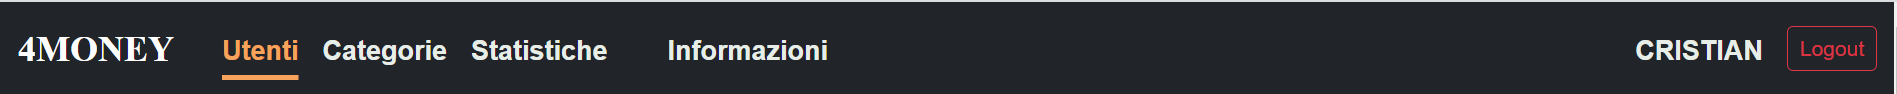
\includegraphics[width=1\linewidth]{navbar_admin.png}
    \caption{Navbar utente amministratore}
    \label{fig:navbar_admin}
\end{figure} \\
Infine la navbar degli amministratori, la quale permette di accedere a pagine loro esclusive, ma anche ad altre simili quali utente nel caso del pulsante "CRISTIAN", il quale riporta il nome del proprietario di questo account di tipo amministratore, e quello di "Logout".
\newpage
\subsection{Home}
\begin{figure}[h]
    \centering
    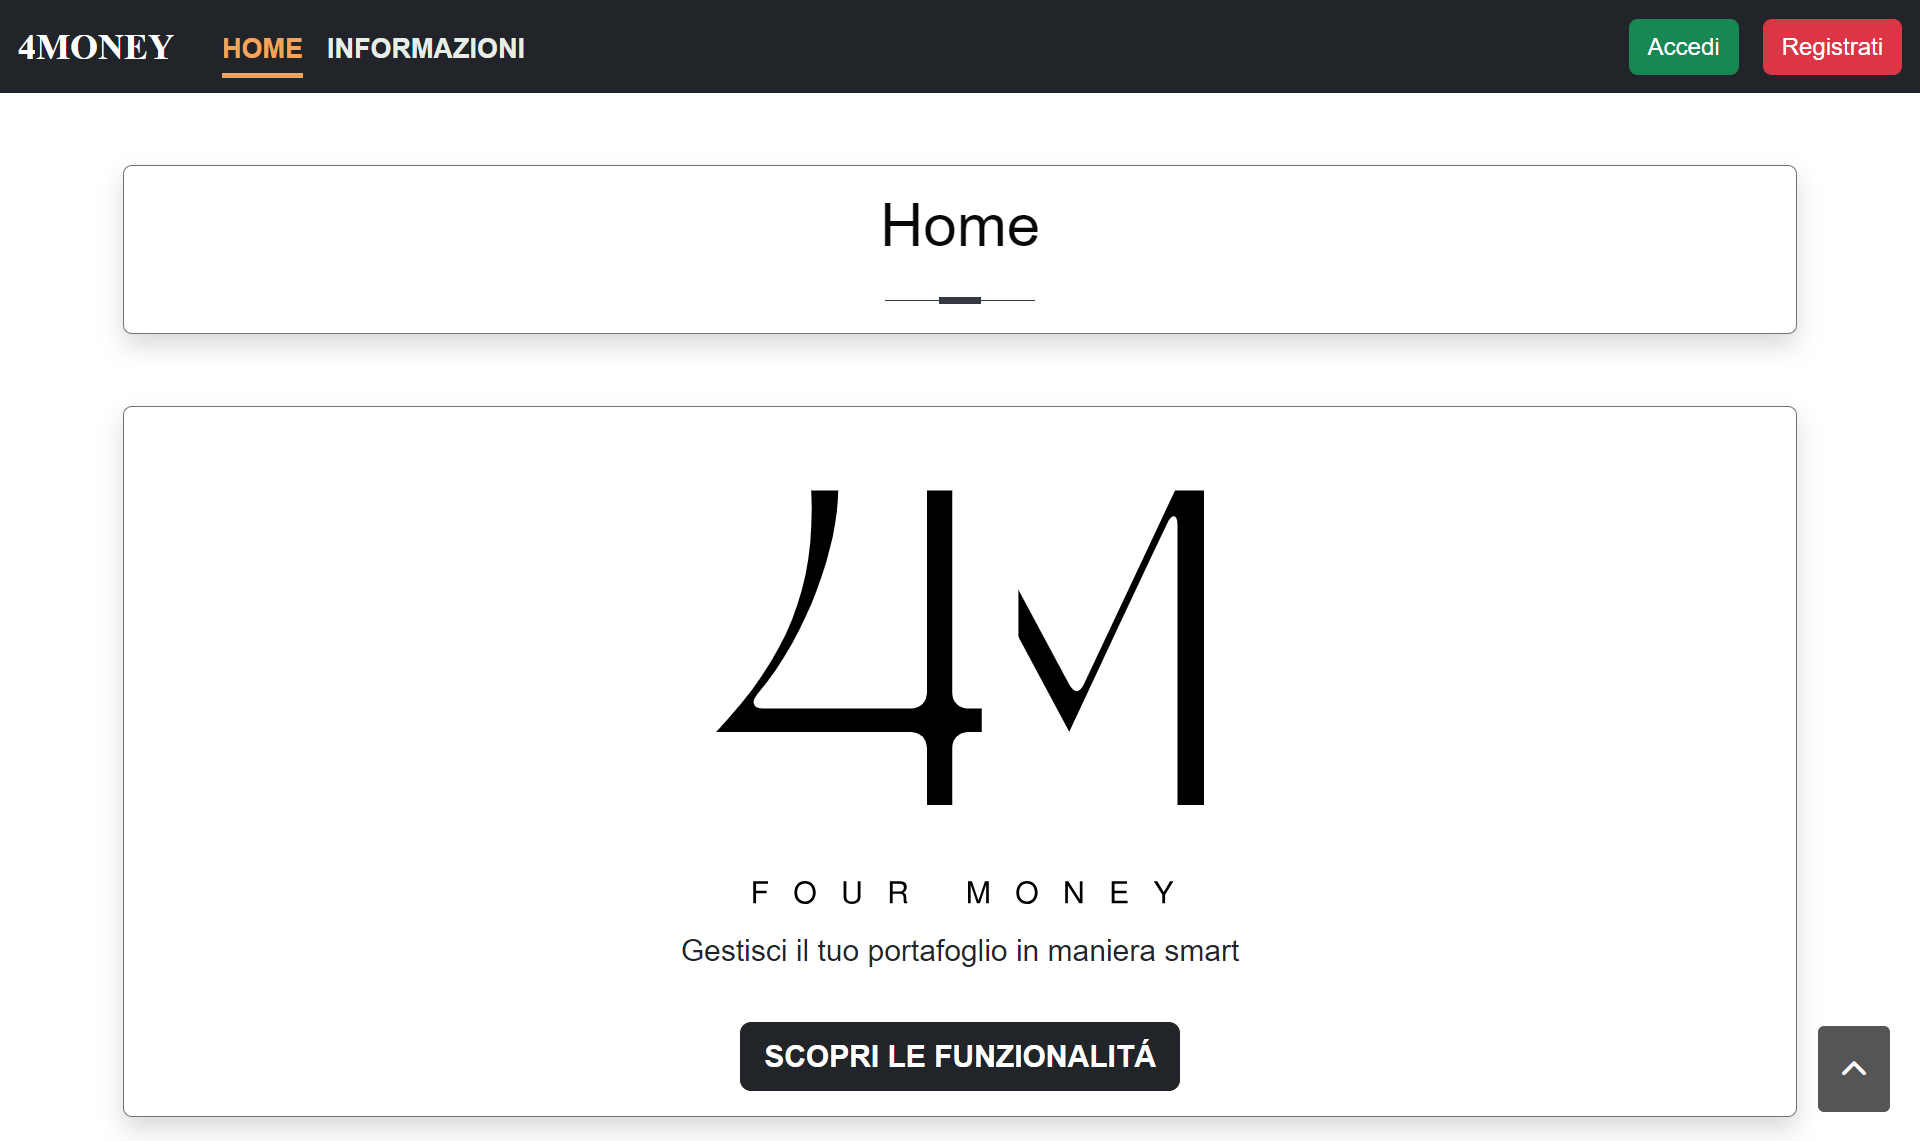
\includegraphics[width=1\linewidth]{home_base.png}
    \caption{Pagina Home}
    \label{fig:home}
\end{figure}
La pagina "Home" è la pagina che funge da "index" dell'applicazione. Le principale funzioni che questa offre sono quelle di facciata per poter passare alle altre pagine attraverso la navbar. Inoltre è presente un pulsante "Scopri le funzionalità" che consente di aprire un sipario come si può vedere nella figura 2.5. La pagina presenta ora le principali funzionalità di 4Money allegando vicino a una rapida descrizione di queste un'immagine esemplificativa. Lo scopo è quello di presentare l'applicazione ai nuovi utenti facendo loro scoprire ciò che possono fare.
\begin{figure}[h]
    \centering
    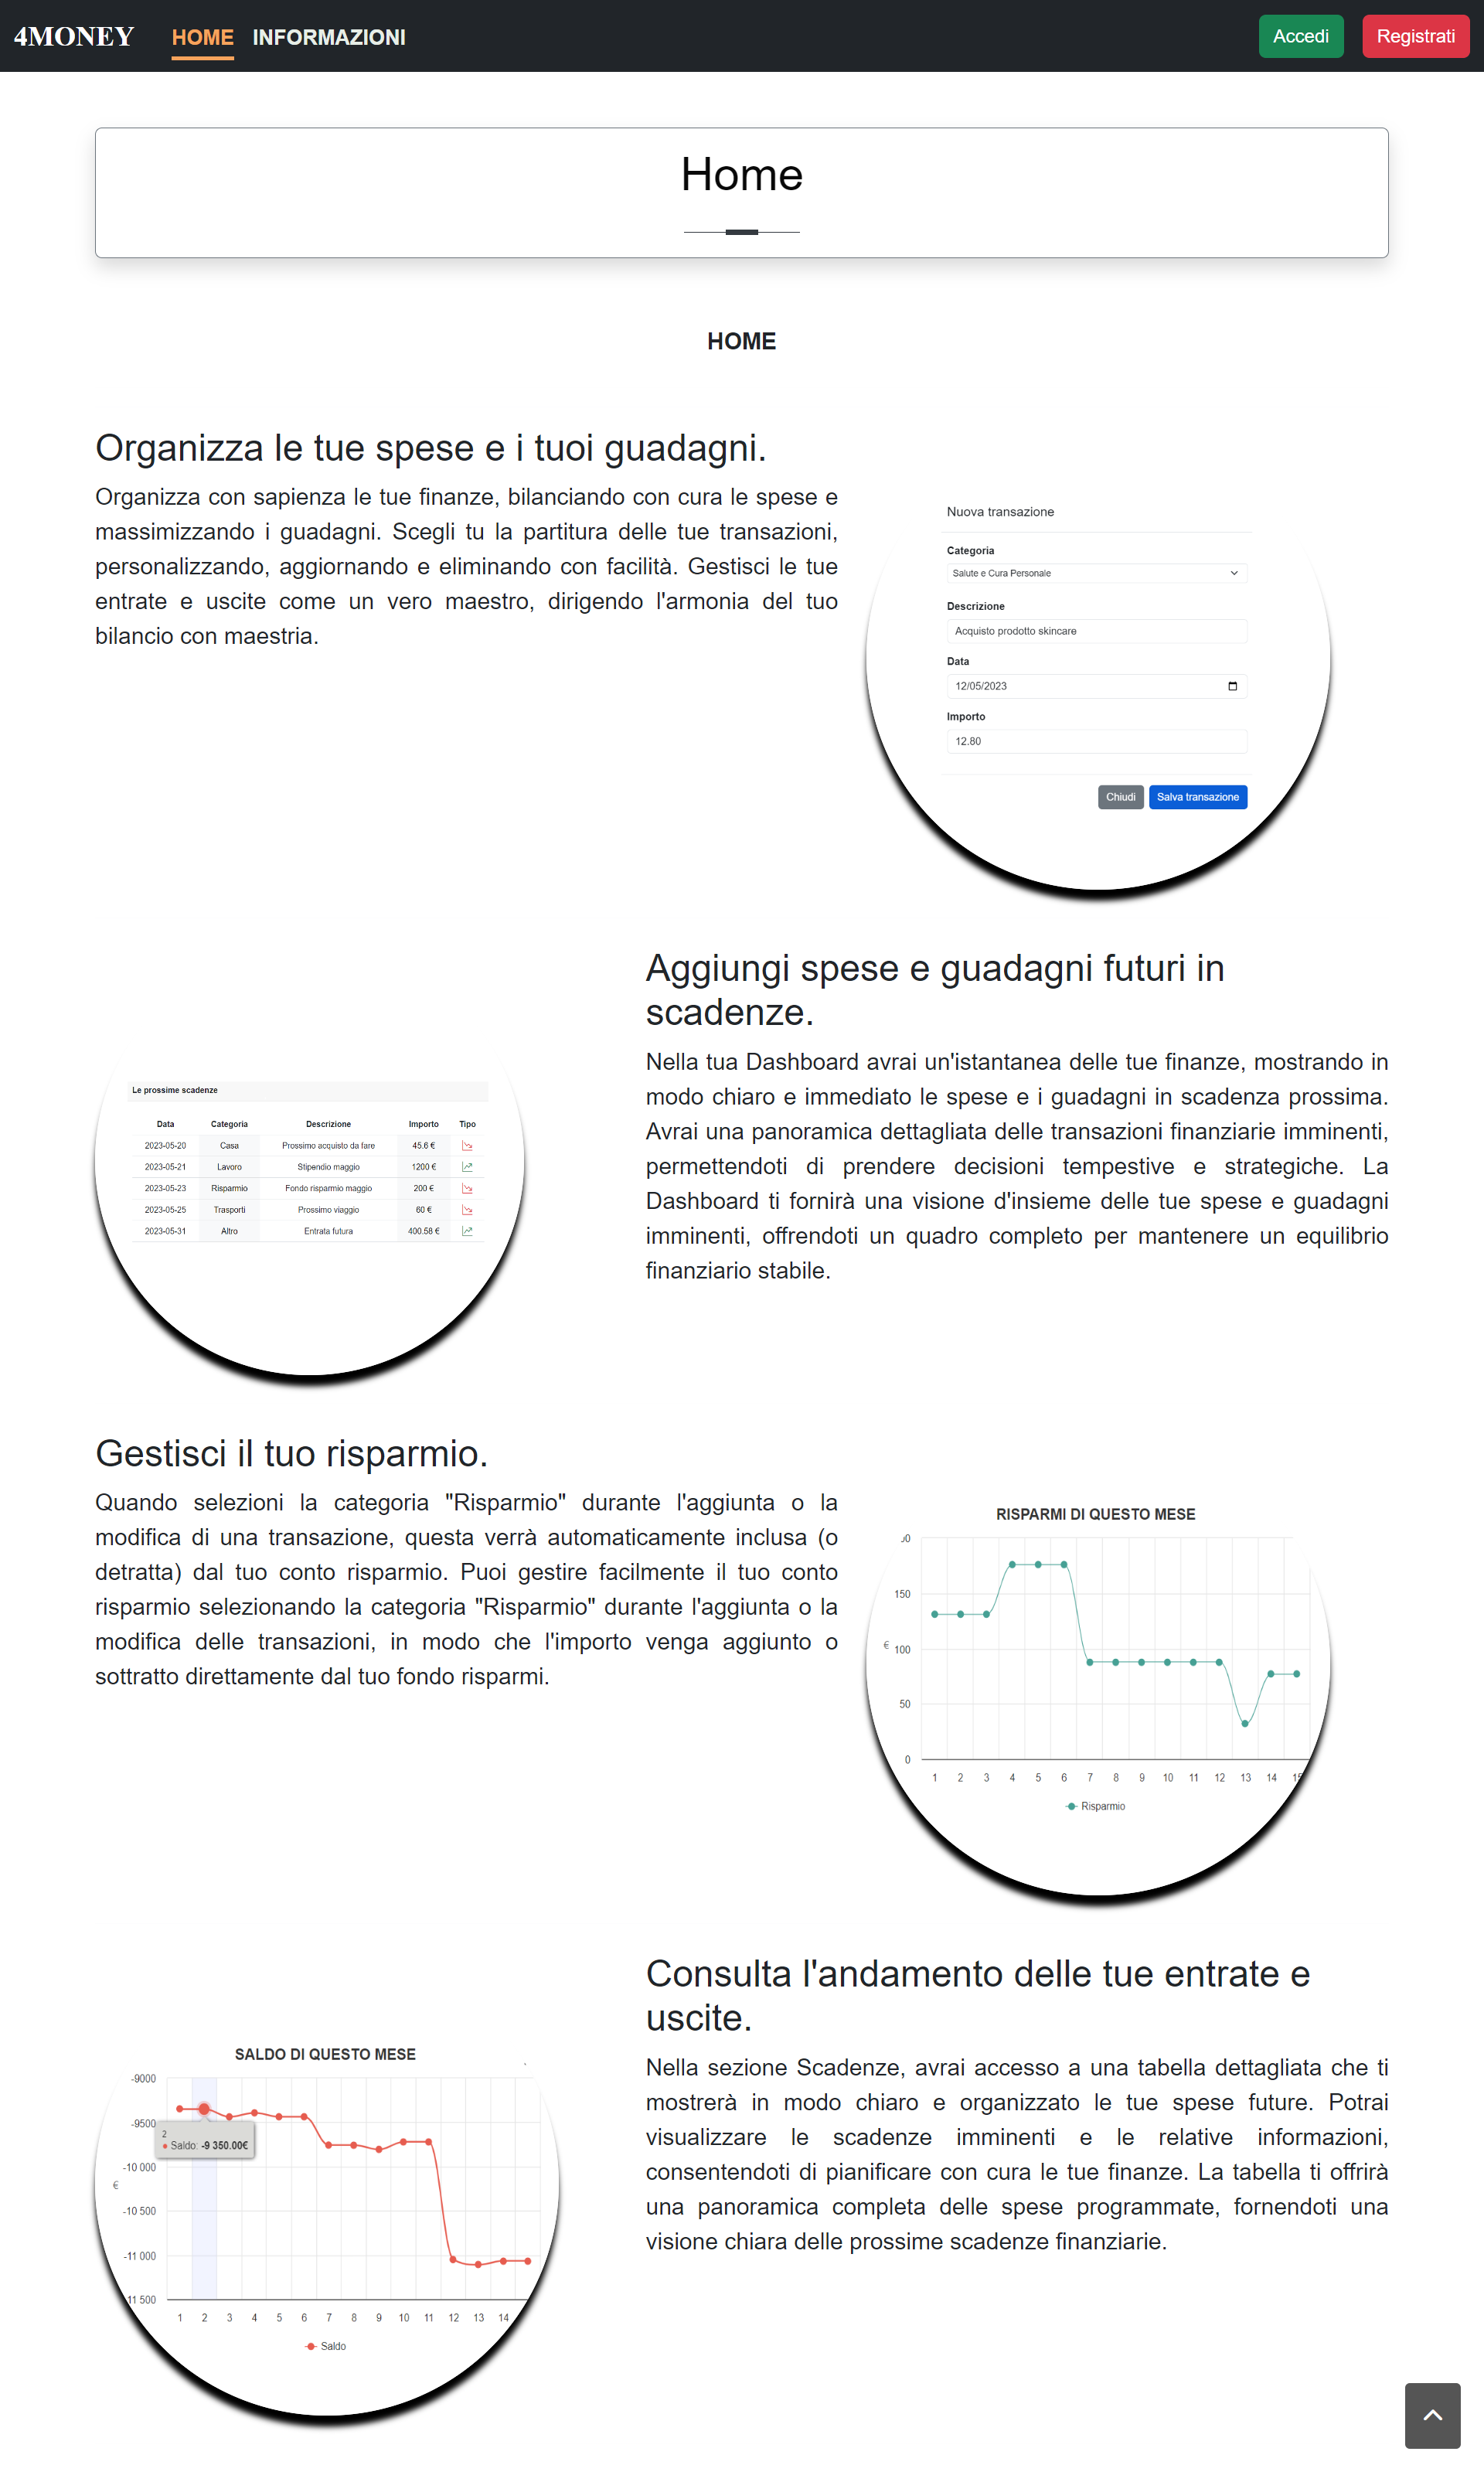
\includegraphics[width=1\linewidth]{home2.png}
    \caption{Home sipario}
    \label{fig:home_sipario}
\end{figure} \\


\end{document}
